\documentclass{beamer}
\usetheme{Goettingen}

\makeatletter
  \setbeamertemplate{sidebar \beamer@sidebarside}
  {
    \beamer@tempdim=\beamer@sidebarwidth%
    \advance\beamer@tempdim by -6pt%
    \vskip4em%
    \insertverticalnavigation{\beamer@sidebarwidth}%
    \vfill
    \hspace{9mm}
\includegraphics[width=1cm]{imagenes/maps.png}
    \ifx\beamer@sidebarside\beamer@lefttext%
    \else%
      \usebeamercolor{normal text}%
      \llap{\usebeamertemplate***{navigation symbols}\hskip0.1cm}%
      \vskip2pt%
    \fi%
  }%

  \ifx\beamer@sidebarside\beamer@lefttext%
    \defbeamertemplate*{sidebar right}{sidebar theme}
    {%
      \vfill%
      \llap{\usebeamertemplate***{navigation symbols}\hskip0.1cm}%
      \vskip2pt}
  \fi

\setbeamertemplate{section in sidebar}%{sidebar theme}
{%
  \vbox{%
    \vskip1ex%
    \beamer@sidebarformat{3pt}{section in sidebar}{\insertsectionheadnumber
~\insertsectionhead}%
  }%
}
\setbeamertemplate{section in sidebar shaded}%{sidebar theme}
{%
  \vbox{%
    \vskip1ex%
    \beamer@sidebarformat{3pt}{section in sidebar shaded}{\insertsectionheadnumber
~\insertsectionhead}%
  }%
}
\makeatother

% contenido de la caratula
\title{\textbf{Path Finder}}
\subtitle{Aplicaci\'on de localizaci\'on para Android}
\author{Almansi, Castro, Vileri\~no}
\date{}

\begin{document}

\begin{frame}
\titlepage
\vspace{-20mm}
\begin{center}
  
\includegraphics[height=2cm]{imagenes/maps.png}
  
\includegraphics[height=2cm]{imagenes/android.png}
\end{center}
\end{frame}

\section{Qu\'e es Path Finder?}

\begin{frame}
\frametitle{Qu\'e es Path Finder?}

    \begin{columns}
        \begin{column}{.7\textwidth}
            \textbf{Path Finder} es una aplicaci\'on para tu dispositivo Android que te acompa\~na a donde vayas, recordando todos los lugares que visit\'as y los recorridos que realiz\'as.
        \end{column}
        \begin{column}{.3\textwidth}\raggedleft
            
\includegraphics[width=2cm]{imagenes/maps.png}
        \end{column}
    \end{columns}

\begin{itemize}
\pause
\item Ubic\'a los puntos de la ciudad por donde anduviste durante el d\'ia, y guard\'a los recorridos que hiciste.
\pause
\item Compart\'i tu ubicaci\'on con tus amigos para que puedan llegar hasta donde est\'as.
\pause
\item Si perdiste de vista o extraviaste tu dispositivo, encontr\'alo desde cualquier tel\'efono o tablet que tengas a mano.
\pause
\item Nunca m\'as pierdas la direcci\'on de un lugar al que quer\'es volver, o un camino que fue dif\'icil encontrar.
\end{itemize}
\end{frame}

\section{C\'omo se usa?}

\begin{frame}
\frametitle{C\'omo se usa?}

Si quer\'es comenzar a guardar tu recorrido, solo necesit\'as instalar \textbf{Path Finder} y crearte una cuenta desde la aplicaci\'on.

\pause
El nombre de usuario y la contrase\~na que elijas, te van a servir despu\'es para consultar tus \'ultimas posiciones desde el mismo dispositivo o desde cualquier otro.

\begin{figure}
	\begin{center}
	  \pause
	  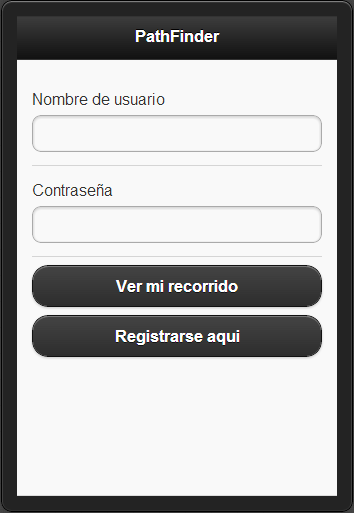
\includegraphics[height=4.5cm]{imagenes/1.png}
	  \hspace{1mm}
	  \pause
	  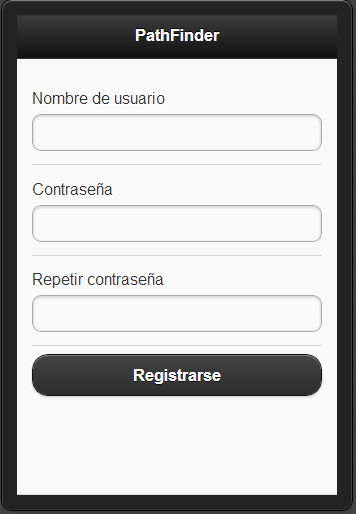
\includegraphics[height=4.5cm]{imagenes/2.png}
	  \hspace{1mm}
	  \pause
	  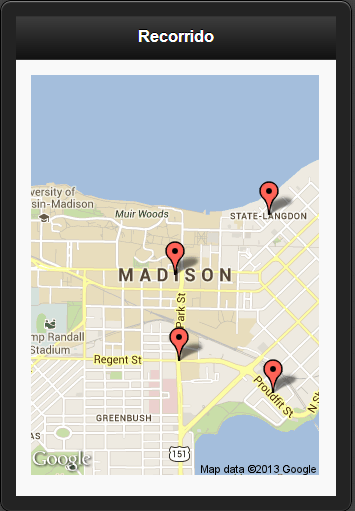
\includegraphics[height=4.5cm]{imagenes/3.png}
	  \hspace{1mm}
	\end{center}
\end{figure}

\end{frame}
\section{C\'omo funciona?}

\begin{frame}

\frametitle{C\'omo funciona?}

\begin{columns}
        \begin{column}{.8\textwidth}
        \begin{itemize}
        	\item La aplicaci\'on se comunica con un servidor dedicado para registrar el nuevo usuario, y a 	partir de ese momento env\'ia los datos de geolocalizaci\'on del dispositivo peri\'odicamente.
        \end{itemize}
        \end{column}
        \begin{column}{.2\textwidth}\raggedleft
            
\includegraphics[width=1.5cm]{imagenes/upload.png}
        \end{column}
    \end{columns}

\pause

\begin{columns}
    \begin{column}{.8\textwidth}
    \begin{itemize}
    	\item Cuando el usuario desea consultar el recorrido de un dispositivo, la aplicaci\'on realiza una solicitud al servidor y se muestran las \'ultimas coordenadas recibidas lanzando la aplicaci\'on de mapas del dispositivo.
    \end{itemize}
    \end{column}
    \begin{column}{.2\textwidth}\raggedleft
        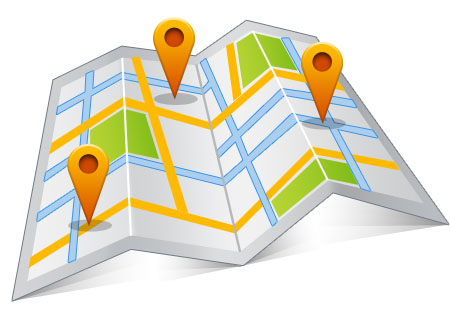
\includegraphics[width=2cm]{imagenes/manypins.png}
    \end{column}
\end{columns}

\pause

\begin{columns}
    \begin{column}{.8\textwidth}
    \begin{itemize}
    	\item Adicionalmente, el dispositivo descarga y muestra tweets con todas las novedades de la aplicaci\'on, publicadas en el Twitter oficial de \textbf{Path Finder}.
    \end{itemize}
    \end{column}
    \begin{column}{.2\textwidth}\raggedleft
        
\includegraphics[width=1.5cm]{imagenes/twitter.png}
    \end{column}
\end{columns}

\end{frame}

\section{Desarrollo futuro}

\begin{frame}

\frametitle{Desarrollo futuro}

\begin{itemize}

\item Lograr que la comunicaci\'on con el servidor y la actualizaci\'on peri\'odica de ubicaci\'on sea independiente de la aplicaci\'on utilizada para visualizar el recorrido de un dispositivo. Es decir, que se ejecute desde que se inicializa el dispositivo, incluso si no se est\'a utilizando la aplicaci\'on.

\pause

\item Permitir m\'ultiples dispositivos para un mismo usuario y contrase\~na.

\pause

\item Dar acceso a mi localizaci\'on y recorrido a otros usuarios de \textbf{Path Finder}; posiblemente mediante la creaci\'on de grupos con permisos para ver la ubicaci\'on de los distintos integrantes del mismo.

\pause

\item Mejor integraci\'on con las redes sociales, permitiendo publicar mi ubicaci\'on en Facebook o Twitter desde la misma aplicaci\'on.

\end{itemize}

\end{frame}


\end{document}